\section{Lyttetests}
\fxnote{Generelt mere nær strukturen på noten. Udførlig argumentation for valg af testparametre.}
For at verificere hvor godt systemet virker, udføres en lyttetest på XX \fxerror{husk tal LS} antal vilkårlige testpersoner. Lyttetesten går ud på at de ud fra et specifikt testsignal skal bedømme hvor de mener at lydkilden er placeret og notere både azimuth, elevation og distance. Testsignalet er en blanding af speak og musik, hvor rækkefølgen er ABABACACADAD \fxnote{Det er vel bare ABAB som testen kaldes?....AB}osv. hvor A henviser til referencepunktet [1,0,0], og B, C og D etc henviser til de forskellige positioner som skal bestemmes af testpersonen.
Testen er udført med musikken afspillet fra en mobiltelefon (hhv en Huawei P10 Lite og en One Plus 2), og høretelefonerne er JBL Everest 300. 
\fxnote{Obs på volumen og hvilken info de skal have LS}

\begin{figure}[h!]
	\centering
	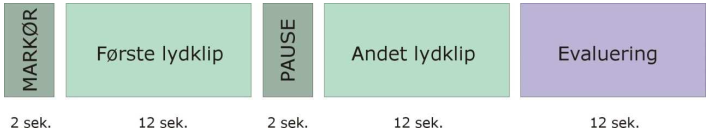
\includegraphics[width=0.7\linewidth]{All_Pics/ABtest}
	\caption{}
	\label{fig:abtest}
\end{figure}
